% % LLNCS macro package for Springer Computer Science proceedings;
% Version 2.21 of 2022/01/12
%
\documentclass[runningheads]{llncs}
%
\usepackage[T1]{fontenc}
% T1 fonts will be used to generate the final print and online PDFs,
% so please use T1 fonts in your manuscript whenever possible.
% Other font encondings may result in incorrect characters.
%

\usepackage{amsmath}
\usepackage{todonotes}
\usepackage{pdfpages}
\usepackage{needspace}

\usepackage[left=2cm,
            right=2cm,
            top=2cm,
            bottom=2cm]{geometry}

\usepackage{graphicx, color, float, subfig}
\captionsetup{font=small,labelfont=bf,labelsep=period,skip=5pt}
\captionsetup[subfloat]{font=scriptsize,labelfont=bf,skip=5pt}

%
\usepackage{hyperref}
\renewcommand\UrlFont{\color{blue}\rmfamily}
\urlstyle{rm}
%

\begin{document}
\title{\fontsize{12}{12}\selectfont Project 2 - Emotion}
\titlerunning{Project 2}
%
\author{Henrik Daniel Christensen\orcidID{hench13@student.sdu.dk} \\Frode Engtoft Johansen\orcidID{fjoha21@student.sdu.dk}}
\authorrunning{Christensen, Johansen} % first names are abbreviated in the running head.
%
\institute{DM873: Deep Learning\\University of Southern Denmark, SDU\\\textit{Department of Mathematics and Computer Science}}
%
\maketitle % typeset the header of the contribution

%%%%%%%%%%%%%%%%%%%%%%%%%%%%%%%%%%%%%%%%%%%
\section{Introduction}
The objective of this project is to develop a deep learning model capable of classifying the sentiment of a given text.
The model will be trained on The \textit{dair-ai/emotion} dataset from Hugging Face, a dataset of 16k tweets labeled with one of 6 emotions: sadness (0), joy (1), love (2), anger (3), fear (4) and surprise (5).
\section{Label Distribution}
We started by analyzing the distribution of the labels in the dataset. The distribution of the labels is shown in Figure \ref{fig:label_dist}.
\begin{figure}[H]
    \vspace*{0.7cm}
    \centering
    \includegraphics[width=0.22\textwidth]{figures/label_dist.png}
    \caption{Distribution of the labels in the dataset.}
    \label{fig:label_dist}
    \vspace*{0.7cm}
\end{figure}
As can be seen, the dataset is very unbalanced, with the majority of the tweets being labeled as joy or sadness. This could potentially lead to the model being biased towards these labels.
\section{Tokenizing and Vocabulary}
Next, we tokenize the text data for that we created a custom RegexpTokenizer which tokenizes the text by only allowing words, numbers and some special characters. Even though the dataset is rather cleaned. Keeping exclasion marks and question marks can be useful for sentiment analysis. To see which words are most common in the dataset, we plot a WordCloud, which can be seen in Figure \ref{fig:wordcloud}.
\begin{figure}[H]
    \vspace*{0.7cm}
    \centering
    \includegraphics[width=0.4\textwidth]{figures/wordcloud.png}
    \caption{WordCloud of the vocabulary.}
    \label{fig:wordcloud}
    \vspace*{0.7cm}
\end{figure}
We see a clear tendency to words accoiated with...

To be sure also all the text was converted to lowercase. We then create a vocabulary of all the unique tokens in the dataset. The vocabulary is then used to convert the text data into sequences of integers. The vocabulary for the training dataset ended up being 15,212 words.

Hereafter, we need to determine the length of the sequences. We do this by plotting the distribution of the lengths of the sequences. The distribution given as a boxplot can be seen in Figure \ref{fig:sequence_length}.
\begin{figure}[H]
    \vspace*{0.7cm}
    \centering
    \includegraphics[width=0.22\textwidth]{figures/sentence_length.png}
    \caption{Distribution of the lengths of the sequences.}
    \label{fig:sequence_length}
    \vspace*{0.7cm}
\end{figure}
From the boxplot, we see that the majority of the sequences have a length of around 20 words. We choose to set the maximum sequence length to 23 words. This means that all sequences longer than 23 words are truncated, and all sequences shorter than 23 words are padded with a special token, '<PAD>', to make them all the same length.


\section{Model 1}
% First, we set out to develop a base model. However, first, we had to decide which image size to use. We choose an image size of 224x224, as this size seems to capture enough details, see page Appendix B - 0.5 Image Size. Also, many of the pretrained models uses the same image size, making our model more comparable to these. Resizing the images has the effect of making training of the model significantly faster and less focused on finer details.

% Next, we had to decide how many layers our model should have. As the task is relatively simple, we decided to use 4 convolutional layers and 3 fully connected layers, including the binary output layer. Since the input images are in color and 224x224 pixels, inputting that image directly into the fully connected layers would result in a $224 \cdot 224 \cdot 3 = 150528$ input size into the model. We would like to reduce this further, so the fully connected layers does not get an input of 150528. The convolution layers extract features, which makes it possible for the neural network to recognise a specific feature no matter where it is in the image, instead of having to learn that feature for every possible position in an image.

% For the loss function, we choose the cross-entropy since it is generally good and popular for classification tasks. For the optimizer, we choose Adam as it combines the strength of several other optimizers. Since we have 4/5 convolutional layers we choose to go with a pretty small kernel size of 3 by 3. A small kernel size is good for preserving details and since we have several convolutional layers it is still possible for us to capture broader features. We use max pooling after each convolutional layer for several reasons. First of all it improves generalization since it focuses on more prominent features. It reduces the dimensionality of the layer, which mean less computation and also reducing complexity so overfitting is less likely. For the activation function, we choose ReLU, as it is the most used activation function for convolutional neural networks.

% Note that the architecture of the model is highly configurable making it easy to experiment with different configurations like different layers, kernels and regularization, see Appendix A - convolutionalNetwork.py. 

% The final base model is provided in Table \ref{tab:base_model}.
% \begin{table}[H]
%     \vspace*{-0.5cm}
%     \centering
%     \begin{tabular}{|l|c|c|c|c|}
%     \hline
%                 & \textbf{Output}           & \textbf{Kernel}   & \textbf{MaxPooling}   & \textbf{Activation}   \\ 
%                 & \textbf{kernels/features} &                   &   &   \\ \hline
%     Conv2D w/   & 32                        & 3x3                   & 2x2                   & ReLU                  \\ \hline
%     Conv2D w/   & 64                        & 3x3                   & 2x2                   & ReLU                  \\ \hline
%     Conv2D w/   & 128                       & 3x3                   & 2x2                   & ReLU                  \\ \hline
%     Conv2D w/   & 256                       & 3x3                   & 2x2                   & ReLU                  \\ \hline
%     Linear w/   & 256                       & -                     & -                     & ReLU                  \\ \hline
%     Linear w/   & 128                       & -                     & -                     & ReLU                  \\ \hline
%     Linear w/   & 2                         & -                     & -                     & -                     \\ \hline
%     \end{tabular}
%     \caption{Base Model.}
%     \label{tab:base_model}
%     \vspace*{-0.8cm}
% \end{table}

% The model was trained for 25 epochs as a start. The learning rate was set to 0.001 as this is a generally good choice. A learning rate that is too small could result in a very slow learning process that might get stuck, and a too big learning rate could result in a local minimum or an unstable learning process. Results of the base model after 25 epochs are shown in Figure \ref{fig:base_model_results}.
% \begin{figure}[H]
%     \vspace*{-0.7cm}
%     \centering
%     \includegraphics[width=0.4\textwidth]{figures/results_base_model.png}
%     \caption{Base Model Results.}
%     \label{fig:base_model_results}
%     \vspace*{-0.7cm}
% \end{figure}

% Clearly, the base model is overfitting, therefore, we need to add some regularization to the model.
\subsection{Model 2: Transformer}
The model is made from the solution to exercise sheet 5. Very few elements have been changed since it follows the pages in the Bishop book closely. The only big changes that has been made to the model itself is added dropout layers and positional encoding. We also experimented with randomly removing 2 tokens from each sentence to increase generalisation but it didn't work. WE also tried adding 2 more linear layers to the transformer block, but this was detrimental to the accuracy so we removed them again.
We chose to use a transformer model as it seems like a good architecture for working with text since it makes words weigh differently depending on which other words are present in the sentence, and with positional encoding also where they are in that sentence. This is important since the meaning of words change depending on other words, and position in sentence.
We used sinusoidal position embedding since this is the positional embedding used in the Bishop book.
The L in the sinusoidal position embedding is 10000. The example in the Bishop book had an L of 30, and some other examples we encountered had an L of 10000. We chose 10000 as the value for L since we encountered it multiple places.\\

We used cross entropy loss as a our loss function since this is a good loss function for classification tasks.
This is the number of heads in the multi head self attention mechanism. d\_model should preferably be divisible by this number so each head computes the same size of input. We chose 8 heads since having too many heads can be inefficient and since we have d\_model of 128, choosing more heads would lead to quite few dimensions per head, which would make it hard for them to capture any useful features.
The mlp factor controls the amount of nodes in the linear layers of the transformer block. We use an mlp factor of 4. This was the default value and decreasing this value hit the performance of the model. Increasing the mlp factor would increase the training time so we decided to not do that.
d\_model is the dimensions of each token. We have a vocabulary of 10336 so we made this pretty big to ensure that each word is able to be uniquely represented. \\

We have 6 layers of transformer blocks. According to the slides, 6 layers is a normal amount of layers and 12 layers is for very large models. We experimented with 6 and 12 layers and found only a small performance increase with 12 layers, but a significant increase in training time, so we decided that we would rather train quicker to test values for other parameters.
When training the transformer models with different parameters we found out that they would quickly overfit, so we needed to generalise the model. To do this we added two dropout layers on the linear layers of the transformer blocks. The dropout chance for the first layer is 50\% and for the second layer is 25\%. We tested with both higher and lower dropout chances and this worked the best.
We chose adam as the optimizer. From the last project our and other peoples takeaway were that adam was a good optimizer in general, and since were not using weight decay, we don't need to use adamW.
We used a learning rate of 0,0003. This was discussed as a good learning rate from the last project, and our experimenting also led us to this learning rate.
We experimented a bit with using weight decay but it did not work well so we decided not to use it in our final model.
When testing different parameters, we used 50 epochs. The transformer models quickly overfitted so we didn't need more epochs. 
We experimented with both L1 and L2 regularisation. L1 regularisation worked the best, and that is probably because it makes some weights go to 0, which indicates those words aren't important. In sentences, some words tells more than other words, so it makes sense that this would be good.

\begin{figure}[H]
    \vspace*{0.7cm}
    \centering
    \includegraphics[width=0.6\textwidth]{figures/transformer_scores.png}
    \caption{Training and validation loss, accuracy, and F1-score for the transformer model.}
    \label{fig:transformer_scores}
    \vspace*{0.7cm}
\end{figure}

\begin{table}[H]
    \vspace*{-0.5cm}
    \centering
    \begin{tabular}{|l|c|c|c|}
        \hline
        Label        & Precision & Recall & F1-Score \\ \hline
        sadness      & 0.89      & 0.82   & 0.85     \\ \hline
        joy          & 0.81      & 0.88   & 0.85     \\ \hline
        love         & 0.68      & 0.59   & 0.63     \\ \hline
        anger        & 0.77      & 0.81   & 0.79     \\ \hline
        fear         & 0.80      & 0.80   & 0.80     \\ \hline
        surprise     & 0.67      & 0.56   & 0.61     \\ \hline\hline
        accuracy     &           &        & 0.81     \\ \hline
        weighted avg & 0.81      & 0.81   & 0.81     \\ \hline
    \end{tabular}
    \caption{Transformer model performance on test set.}
    \label{tab:rnn_lstm_model_test}
    \vspace*{-0.8cm}
\end{table}

Despite a lot of parameter tuning, we could not get the transformer model to get a better performance. We even tried adding extra linear layers in the transformer block, and removing random words from the sentences for better generalisation.

\section{Analysis and Final Prediction}
% The reg\_4 model is now applied to the test set to evaluate its performance. The test accuracy is summarized in Table \ref{tab:prediction}.

% \begin{table}[H]
%     \centering
%     \begin{tabular}{|c|c|}
%         \hline
%         \textbf{Test Accuracy using Reg4 model} \\ \hline
%         91.5\% \\ \hline
%     \end{tabular}
%     \caption{Test Accuracy using Reg4 Model.}
%     \label{tab:prediction}
% \end{table}

% Some of the misclassified and correctly classified images are given in Figure \ref{fig:prediction}.
% \begin{figure}[H]
%     \vspace*{-0.7cm}
%     \centering
%     \includegraphics[width=1\textwidth]{figures/predict_images.png}
%     \caption{Misclassified and correctly classified images.}
%     \label{fig:prediction}
%     \vspace*{-0.7cm}
% \end{figure}

% From the misclassified images, we see that may some more data augmentation could be applied to improve the model's performance. For example, the cat that rotate its head by almost 90 degrees. Moreover, the model may be improved by adding more crop-scale augmentation.
\section{Pretrained Model (RoBERTa)}
% To see how good our model performs compared to a well-known model, we used the pretrained model 'AlexNet'.
% This model is pretrained on the ImageNet dataset, which contains 1.2 million images and 1000 classes, also including cats and dogs.
% However, to use the pretrained model for this binary classification task, the output layer is modified.
% The results of the pretrained model after 20 epochs are shown in Figure \ref{fig:results_alexnet}. The test accuracy is summarized in Table \ref{tab:alexnet}.

% \begin{figure}[H]
%     \vspace*{-0.7cm}
%     \centering
%     % Subfigure 1:
%     \subfloat[Loss and Accuracy scores using AlexNet.\label{fig:results_alexnet}]{\includegraphics[width=0.4\textwidth]{figures/results_alexnet.png}}
%     \hspace{0.4cm}
%     \subfloat[Test Accuracy using AlexNet.\label{tab:alexnet}]{
%         \raisebox{\height}{    
%         \begin{tabular}{|c|}
%             \hline
%             \textbf{Test Accuracy using AlexNet} \\ \hline
%             93.5\% \\ \hline
%         \end{tabular}}}
%     \caption{AlexNet results.}
%     \label{fig:alexnet}
%     \vspace*{-0.7cm}
% \end{figure}


% As expected the pretrained model performs sligtly better than our model. However, AlexNet also is trained on a much larger dataset and has a lot more parameters ($\sim 57$ million) compared to our model ($\sim 21$ million). The feature maps look pretty similar to our model, but is less interpretable, probably generalizing better to other objects.
\section{Conclusion}
We constructed two different models to complete the task, a recurrent neural network with LSTM and 256 hidden units, and a transformer model with 6 transformer layers. The recurrent neural network had the best test accuracy of 83\%, while the transformer model had a test accuracy of 81\%. We tried using a pretrained model distilBERT on our task to see how it would fare. It got a test accuracy of 89\%. As expected our models were worse. This can be explained by the fact that distilBERT has more parameters and a much bigger training set than our models. 

Overall we are satisfied with our result but it could have been improved. Initially an accuracy of 83\% seems quite bad, but even the pretrained model had a test accuracy of less than 90\% so compared to that, it does not seem too bad. 

\subsection{Individual Contributions}
\begin{table}[H]
    \centering
    \begin{tabular}{|l|l|l|}
    \hline
                    & \textbf{Henrik Daniel Christensen}    & \textbf{Frode Engtoft Johansen} \\ \hline
    \textbf{Code}   & Task 1, 2, 5                          & Task 3, 4\\ \hline
    \textbf{Report} & Section 1, 2, 3, 4.1, 6                 & Section 4.2, 5, 7 \\ \hline
    \end{tabular}
    \caption{Individual contributions.}
    \label{tab:individual_contributions}
\end{table}


%%%%%%%%%%%%%%%%%%%%%%%%%%%%%%%%%%%%%%%%%%%

%Appendices
\newpage
\appendix
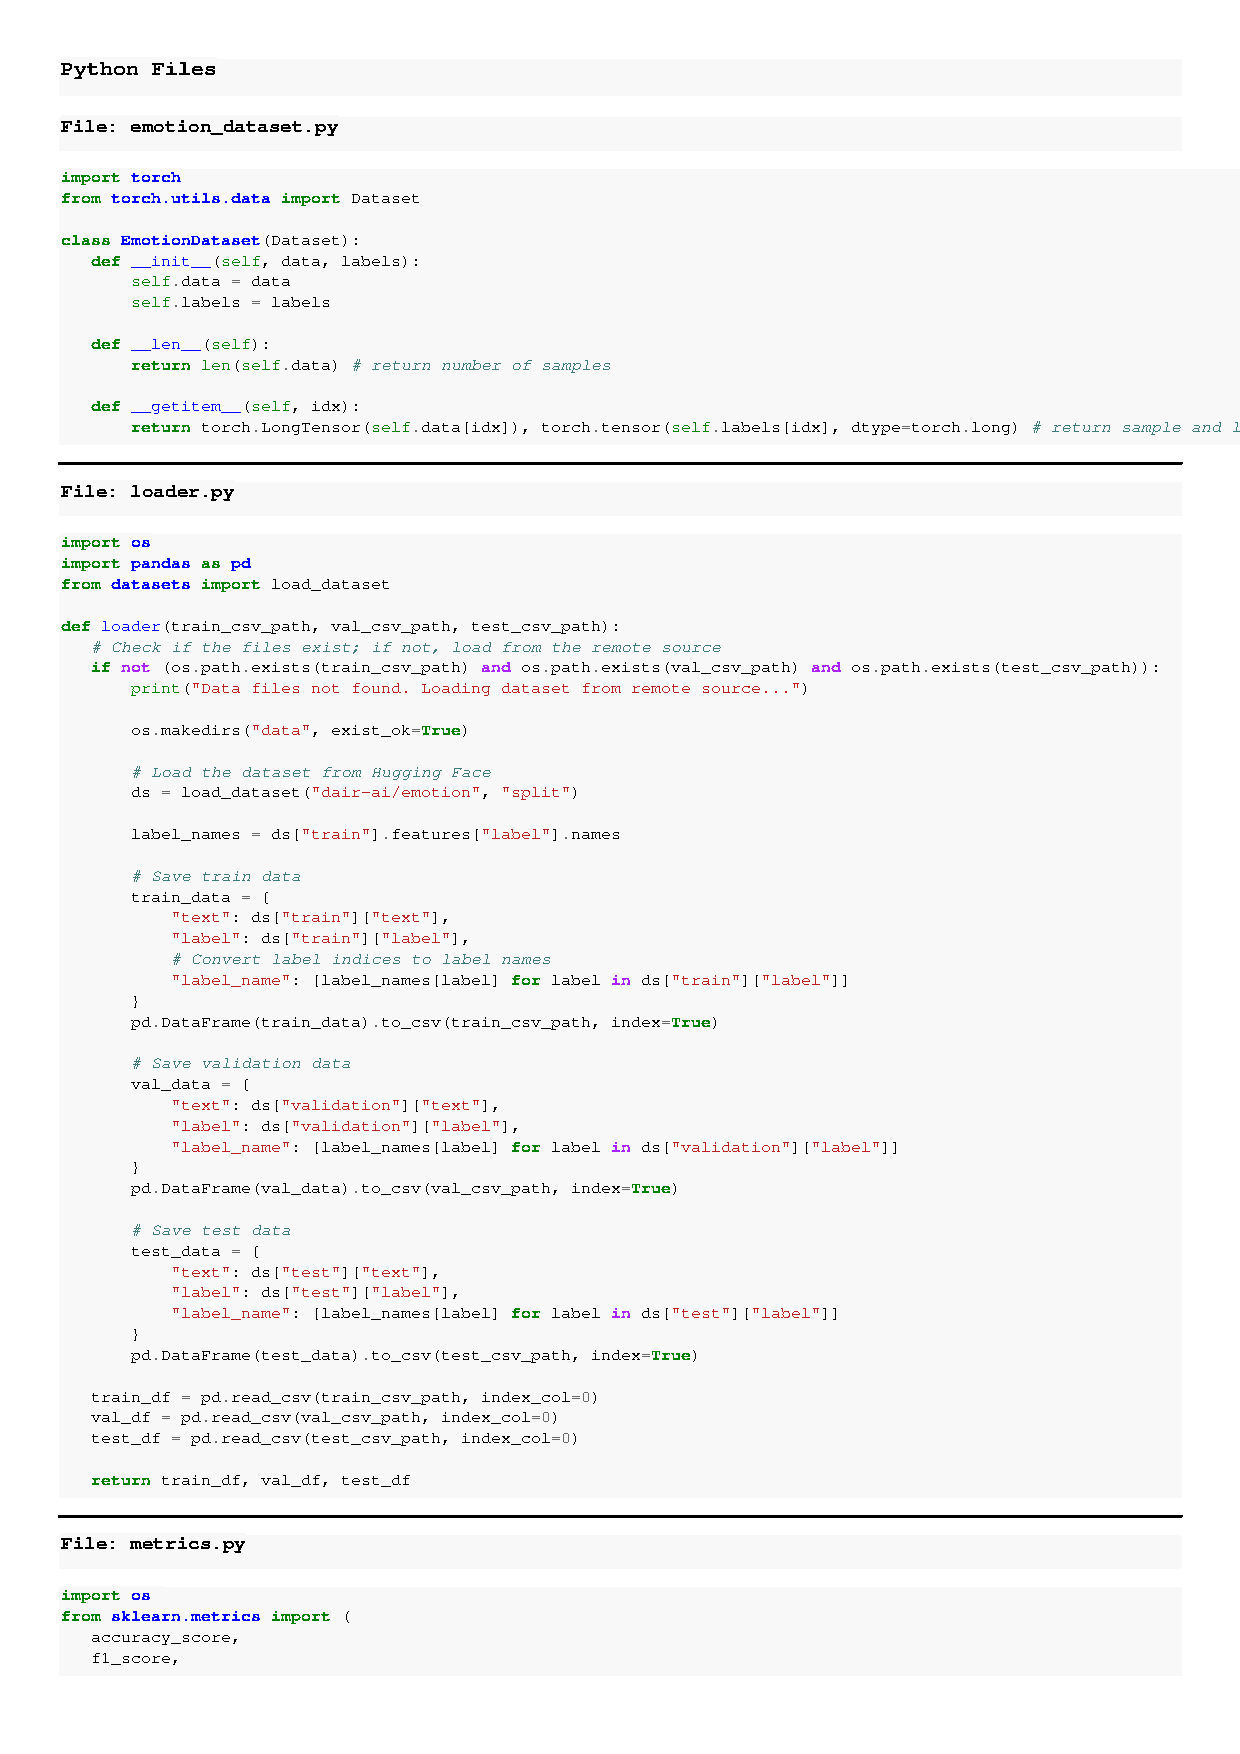
\includepdf[pages=1,scale=.85,pagecommand={\section{Code}\label{app:code}}]{../src/code.pdf}
\includepdf[pages=2-,scale=.85,pagecommand={}]{../src/code.pdf}
\includepdf[pages=1,scale=.85,pagecommand={\section{Notebook}\label{app:notebook}}]{../src/notebook.pdf}
\includepdf[pages=2-,scale=.85,pagecommand={}]{../src/notebook.pdf}

% \bibliographystyle{base/splncs04}
% \newpage
% \bibliography{base/references}
%%%%%%%%%%%%%%%%%%%%%%%%%%%%%%%%%%%%%%%%%%%
\end{document}